\chapter{Point Attractor Network on a Neuromorphic Chip}

\section{Bias (parameters) on chip}
\subsection{Linear properties of bias settings}
% board parameter linear properties
Each core on the chip share the same synapse properties. Before tuning the parameters to obtain a point attractor behaviour, the relation between the bias we set and the bias the board applied is investigated.\\

Each bias contains two values, one coarse value ranging from 0-7 and a fine value ranging from 0-255.
The given coarse value and fine value will be translated into a linear value which will then be applied on the chip.\\

The relationship between the coarse value and fine value is shown in figure \ref{fig:cf2l}.
Figure \ref{fig:cf2l_absolute} shows that in each coarse values settings with varying fine values, the translated linear value all started from 0, the higher the coarse value, the higher linear value range the bias can reach by tuning the fine values.
Figure \ref{fig:cf2l_absolute2} shows all the translated bias values in one coarse set are linear to the fine values with different slopes.
A log scale plot as shown in figure \ref{fig:cf2l_log} is made to make the relationship between different coarse sets more readable.\\


% fitting
The slopes of each coarse set are measured and listed in table \ref{tab:cf2l}.
After taking the logarithm of the slope, a linear relationship is found as shown in figure \ref{fig:c2f_slopes}.

Therefore, the coarse and fine value bias translation is approximated by a function  $y=5.88e^{2.04c}f$, where $c$ represents coarse value and $f$ represents fine value). The fitted slope and corresponding bias settings are plotted into the figures and find a good fit between the measurement of board 020 and the curve fitting.

% Table generated by Excel2LaTeX from sheet 'parameters copy'
\begin{table}
	\centering
	\begin{tabular}{lcccccccc}
		\toprule
		coarse & 0     & 1     & 2     & 3     & 4     & 5     & 6     & 7 \\
		\midrule
		slope & 5.88  & 41.18 & 321.57 & 2549.02 & 19607.84 & 156862.75 & 1254901.96 & 9411764.71 \\
		\bottomrule
	\end{tabular}%
	\caption{The slope of bias values under each coarse set.}
	\label{tab:cf2l}%
\end{table}%


\begin{figure}
	\begin{subfigure}{\textwidth}
		\centering
		% include first image
		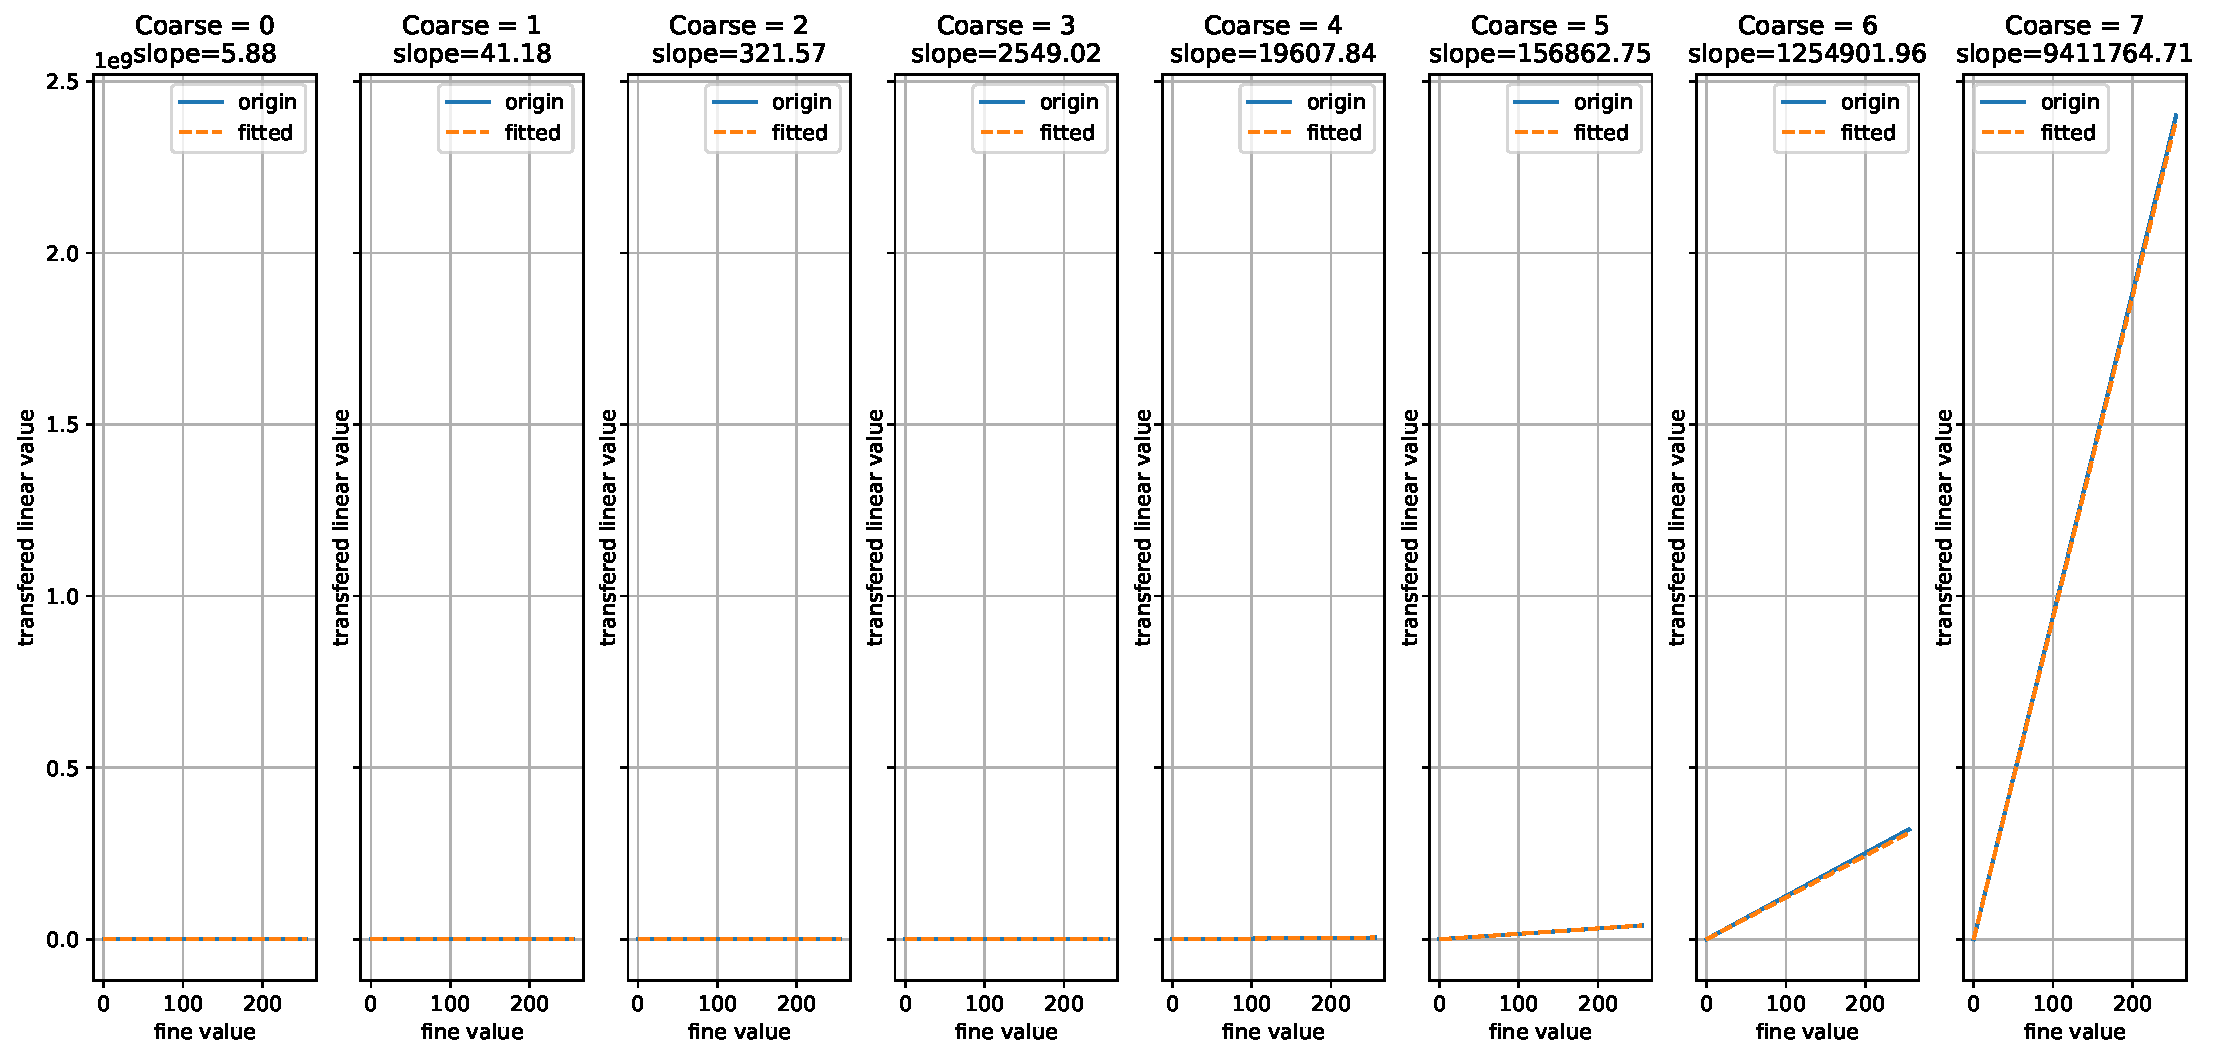
\includegraphics[page=1, width=\columnwidth]{./img/implementation/cf2linear.pdf}
		\caption{shared y scale representation}
		\label{fig:cf2l_absolute}
	\end{subfigure}
	\begin{subfigure}{\textwidth}
		\centering
		% include second image
		\includegraphics[page=2, width=\columnwidth]{./img/implementation/cf2linear.pdf}
		\caption{flexible y scale representation}
		\label{fig:cf2l_absolute2}
	\end{subfigure}
	\begin{subfigure}{\textwidth}
		\centering
		% include second image
		\includegraphics[page=3, width=\columnwidth]{./img/implementation/cf2linear.pdf}
		\caption{log y scale representation}
		\label{fig:cf2l_log}
	\end{subfigure}
	
	\caption{cf to linear values of board 000020, fitted with function $y=5.88e^{2.04c}f$ (c: coarse value, f: fine value)}
	\label{fig:cf2l}
\end{figure}

\begin{figure}
	\centering
	\includegraphics[page=4, width=\columnwidth]{./img/implementation/cf2linear.pdf}
	\caption{Slope of bias values under different coarse settings, fitted with $y=5.88e^{2.04c}$}
	\label{fig:c2f_slopes}
\end{figure}


% synapse 在相同设置的情况下 neuron firing的对比是否相同
\subsection{Synapse properties on chip}

\begin{figure}
	\begin{subfigure}{.5\textwidth}
		\centering
		% include first image
		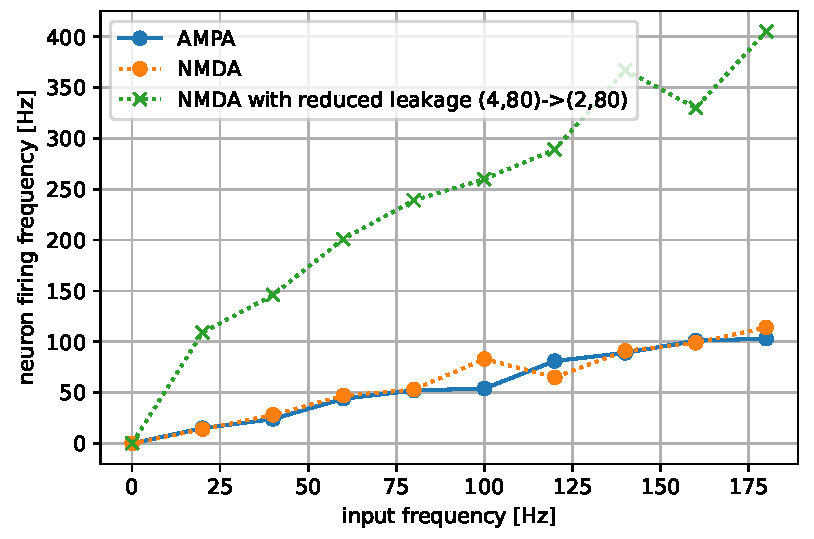
\includegraphics[page=1, width=\columnwidth]{./img/implementation/synapse.pdf}
		\caption{Frequency range 0-180Hz}
		\label{fig:synapse_1}
	\end{subfigure}
	\begin{subfigure}{.5\textwidth}
		\centering
		% include second image
		\includegraphics[page=2, width=\columnwidth]{./img/implementation/synapse.pdf}
		\caption{Frequency range 0-1800Hz}
		\label{fig:synapse_2}
	\end{subfigure}
	\caption{The neuron FF curve with same AMPA, NMDA parameters applied.}
	\label{fig:synapse}
\end{figure}

\begin{table}
	\centering
	\begin{tabular}{ccccccccc}
		\toprule
		NG\_c & NG\_f & NL\_c & NL\_f & NR\_c & NR\_f & aG\_c & aG\_f & aL\_c \\
		\midrule
		5     & 80    & 4     & 80    & 4     & 128   & 4     & 80    & 4 \\
		\midrule
		aL\_f & aW\_c & aW\_f & nG\_c & nG\_f & nL\_c & nL\_f & nW\_c & nW\_f \\
		\midrule
		80    & 7     & 100   & 4     & 80    & 4     & 80    & 7     & 100 \\
		\bottomrule
	\end{tabular}%
	\label{tab:synapse}%
	\caption{Comparison of neuron firing behaviour by giving AMPA and NMDA the same parameter.(N: Neuron, a: AMPA, n: NMDA, G:  gain, L: leakage, R: refractory period, W: weight, c: coarse, f: fine)}
\end{table}%
% TODO 增加 weight 看FF
As shown in figure \ref{fig:synapse}, given the same parameter settings for AMPA and NMDA as shown in table  \ref{tab:synapse}, the firing rate of the neuron seems to be identical, therefore, different from the brian2 software simulation, the two synapse on board is considered to be the same. \\

To obtain a slow NMDA receptor behaviour given the same weight parameter, further reducing leakage current is required. The effect of reducing the leakage current is shown in the figure \ref{fig:synapse}. Both reduction of leakage current and increase the weight can help increase the neuron firing rate.

As shown in figure \ref{fig:synapse_2}, by increasing the input frequency range from 180 to 1800Hz, the neuron refractory period effect appears where a neuron firing rate saturation shows. 


\subsection{Parameter tuning}
% applied parameters
\begin{table}
	\centering
	\begin{tabular}{cccccccc}
		\midrule
		chip  & core  & NG\_c & NG\_f & NL\_c & NL\_f & NR\_c & NR\_f \\
		\midrule
		0     & 0     & 5     & 80    & 4     & 80    & 4     & 128 \\
		0     & 1     & 5     & 80    & 4     & 80    & 4     & 128 \\
		0     & 2     & 5     & 80    & 4     & 80    & 4     & 128 \\
		\midrule
		chip  & core  & aG\_c & aG\_f & aL\_c & aL\_f & aW\_c & aW\_f \\
		\midrule
		0     & 0     & 4     & 80    & 4     & 80    & 4     & 80 \\
		0     & 1     & 4     & 80    & 4     & 80    & 6     & 50 \\
		0     & 2     & 4     & 80    & 4     & 80    & 5     & 200 \\
		\midrule
		chip  & core  & nG\_c & nG\_f & nL\_c & nL\_f & nW\_c & nW\_f \\
		\midrule
		0     & 0     & 4     & 80    & 4     & 80    & 4     & 80 \\
		0     & 1     & 4     & 80    & 4     & 80    & 3     & 50 \\
		0     & 2     & 4     & 80    & 4     & 80    & 7     & 50 \\
		\midrule
		chip  & core  & AG\_c & AG\_f & AL\_c & AL\_f & AW\_c & AW\_f \\
		\midrule
		0     & 0     & 4     & 80    & 4     & 80    & 4     & 80 \\
		0     & 1     & 4     & 80    & 2     & 200   & 7     & 200 \\
		0     & 2     & 4     & 80    & 4     & 80    & 7     & 20 \\
		\bottomrule
	\end{tabular}%
	\label{tab:parameter}%
	\caption{Parameter settings (N: Neuron, a: AMPA, n: NMDA, A: GABA\_A, G:  gain, L: leakage, R: refractory period, W: weight, c: coarse, f: fine)}
\end{table}%
% visualized parameters
\begin{figure}
	\begin{subfigure}{\textwidth}
		\centering
		% include first image
		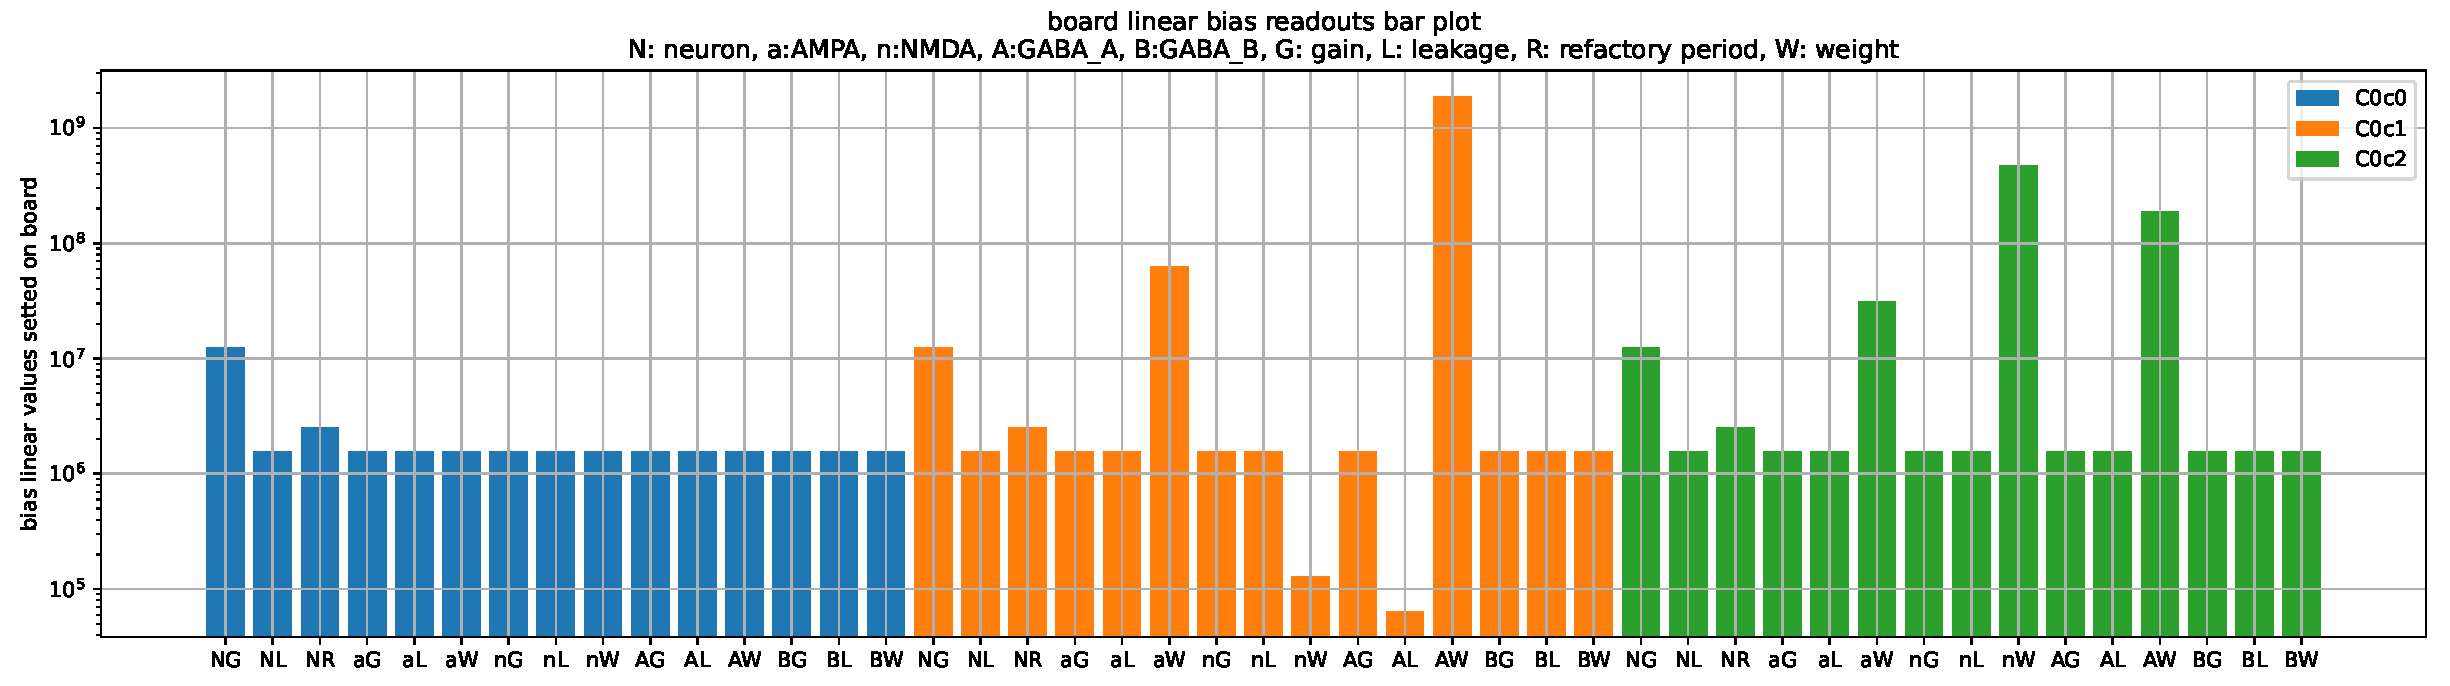
\includegraphics[page=1, width=\columnwidth]{./img/implementation/bias_readouts.pdf}
		\caption{Bias values bar plot}
		\label{fig:biasOnBoard_bar}
	\end{subfigure}
	\begin{subfigure}{\textwidth}
		\centering
		% include second image
		\includegraphics[page=2, width=\columnwidth]{./img/implementation/bias_readouts.pdf}
		\caption{Bias values comparison on curve}
		\label{fig:biasOnBoard_online}
	\end{subfigure}
	\caption{Applied bias values on board.(N: Neuron, a: AMPA, n: NMDA, A: GABA\_A, G:  gain, L: leakage, R: refractory period, W: weight, c: coarse, f: fine)}
	\label{fig:biasOnBoard}
\end{figure}

% describe the parameter tuning
The detailed parameters applied on board to obtain a point attractor behaviour is shown in table \ref{tab:parameter}. To simplify, the major parameters tuned for core 1 is AMPA weight, NMDA weight, GABA\_A weight and leakage; the major parameters tuned for core 2 is AMPA weight and GABA\_A weight as visualized in figure \ref{fig:biasOnBoard}.\\

To obtain a point attractor behaviour, the AMPA weight for core 1 is set as (6,50), NMDA weight is set as (3, 50), GABA\_A weight is set as (7, 200) and GABA\_A leakage is set as (2, 200).

The intension behind the settings is to enhance the $E_{att}$ population recurrent connections and balance the $E_{bkg}$ population influence.
Besides, to increase the sensitivity of E population to the inhibitory afferent.\\

The AMPA weight for core 2 is set as (5, 200), GABA\_A is set as (7, 20). 

The intension behind the settings is to enhance the I population recurrent connections and increase the sensitivity to the excitatory afferent. In comparison with E population, the I population therefore obtain a faster response.

\section{Architecture of the Point Attractor}
\begin{figure}
	\centering
	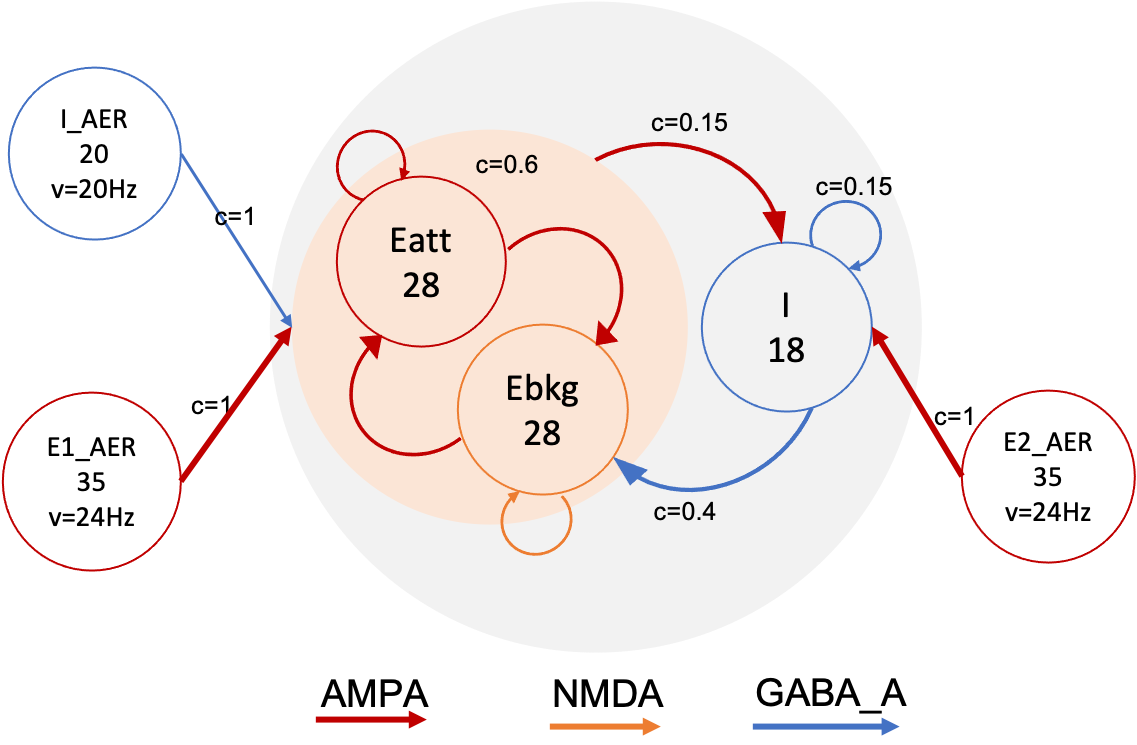
\includegraphics[width=\columnwidth]{./img/implementation/network_structure.png}
	\caption{Network structure implemented on DYNAPSE board. The neurons in the gray circle is implemented on chip. The AER stimuli are from FPGA spike generator. }
	\label{fig:NNstructure}
\end{figure}

% network structure
A network structure that is similar to the point attractor network mentioned above in Chapter \ref{cpt:introduction} is implemented on the DYNAPSE board as shown in figure \ref{fig:NNstructure}. The DYNAP-SE1 board is a neuromorphic chip which has 4 chips and each chip contains 4 cores featuring 256 silicon neurons.\\

% synapses
By using two types of excitatory receptors (synapse) "AMPA" and "NMDA" on board, the potentiated excitatory synapse and depressed excitatory synapse are represented. 
Besides, the GABA\_A receptor (synapse) on board is used to represent the inhibitory synapse.

% inter-connections
The $E_{att}$ and $E_{bkg}$ populations connections and E and I population connection is similar to the connection mentioned in the literature \cite{giudiceRobustWorkingMemory2012}.\\

% the difference
However, due to the limitation of hardware supported number of synapses that each neuron can be connected to. It is hard to build such a large network with 48 $E_{att}$ neurons and 48 $E_{bkg}$ neurons on this board. Therefore, a scaling of this network is done by using a factor 0.6 to ensure the connection is implementable on this chip.
As a result, the number of $E_{att}$ and $E_{bkg}$ neurons is scaled to 28 and the number of I neurons is scaled to 18. With this scaling, the connection can be built successfully with the same connection probabilities mentioned in the literature.\\

Besides, instead of using big number of neurons for the input Poisson stimuli and with a very small connection probability. A small number of neuron is chosen and a probability of 1 is given for establishing the connection between the input spike generators and E, I neuron populations.

\section{Mapping the network on the DYNAPSE board}

\begin{figure}
	\begin{subfigure}{0.5\textwidth}
		\centering
		% include first image
		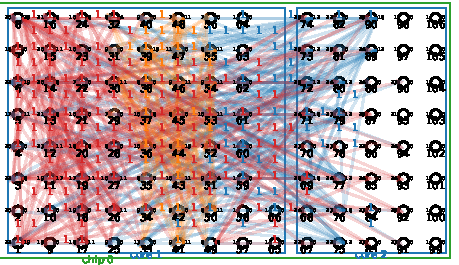
\includegraphics[page=1, width=\columnwidth]{./img/implementation/network.pdf}
		\caption{All the inter-connections between E and I neuron populations.}
		\label{fig:NNonboard1}
	\end{subfigure}
	\begin{subfigure}{0.5\textwidth}
		\centering
		% include second image
		\includegraphics[page=2, width=\columnwidth]{./img/implementation/network.pdf}
		\caption{All AMPA connections between E and I neuron populations.}
		\label{fig:NNonboard2}
	\end{subfigure}
	\begin{subfigure}{0.5\textwidth}
		\centering
		% include second image
		\includegraphics[page=3, width=\columnwidth]{./img/implementation/network.pdf}
		\caption{All NMDA connections inside $E_{bkg}$ neuron population.}
		\label{fig:NNonboard3}
	\end{subfigure}
	\begin{subfigure}{0.5\textwidth}
		\centering
		% include second image
		\includegraphics[page=4, width=\columnwidth]{./img/implementation/network.pdf}
		\caption{All GABA\_A connections inside I neuron population and between E and I neuron population.}
		\label{fig:NNonboard4}
	\end{subfigure}
	\begin{subfigure}{\textwidth}
		\centering
		% include second image
		\includegraphics[page=5, width=0.9\columnwidth]{./img/implementation/network.pdf}
		\caption{Excitatory spike generator connected to all the $E_{att}$ population and I neuron population.with AMPA}
		\label{fig:NNonboard5}
	\end{subfigure}
	\begin{subfigure}{\textwidth}
		\centering
		% include second image
		\includegraphics[page=6, width=0.9\columnwidth]{./img/implementation/network.pdf}
		\caption{Inhibitory spike generator connected to $E_{att}$ neurons with GABA\_A}
		\label{fig:NNonboard6}
	\end{subfigure}
	\caption{Connections implemented on board (AMPA: red, NMDA: orange, GABA\_A: blue).}
	\label{fig:NNonboard}
\end{figure}

The detailed on board connections is visualized in the figure \ref{fig:NNonboard}. \\

% population, core, number of neurons
As shown in the figure, there are 106 neurons are allocated in core 0 for generating the spike input. The 56 excitatory neurons are allocated in core 1 and 18 inhibitory neurons are allocated in core2. \\

% inter-connection methods
There are three types of connections between the neurons that has been applied as shown in figure \ref{fig:NNonboard1}, \ref{fig:NNonboard2}, \ref{fig:NNonboard3} and \ref{fig:NNonboard4}.
Different type of connection is shown with different colours where red represents AMPA, orange represents NMDA and blue represents GABA\_A. 

The incoming connections is shown on the left port of the neuron and the output connections is shown on the right port of the neuron. The number of fan-in of each neuron is physically limited to 64 and the numbers of input and output connections are displayed on left and right port of the neurons.\\

% recurrent connection
When a recurrent connection appears, the neuron will connect its left and right port, the number above the line shows the number of synapse between two nodes.\\

% spike input 
The input Poisson stimuli are generated by spike generators. Each of them are connected to each neuron in corresponding populations (E or I population).
There are two types of input stimuli transmission, one is transmitted with excitatory connections AMPA as shown in figure \ref{fig:NNonboard5}, and the other is transmitted with inhibitory connections NMDA as shown in figure \ref{fig:NNonboard6}. 

\section{Results}

\begin{figure}
	\begin{subfigure}{\textwidth}
		\centering
		% include first image
		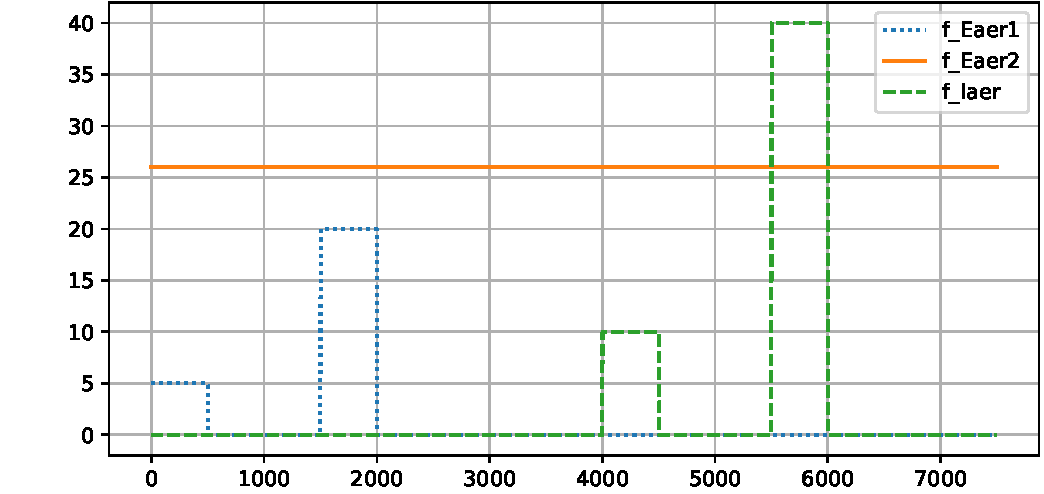
\includegraphics[page=1, width=0.95\columnwidth]{./img/behavior/input_stimuli.pdf}
		\caption{Stimuli of the AER input. (Poisson spike train at different frequencies) (x: time [ms], y: frequency [Hz])}
		\label{fig:spike_input}
	\end{subfigure}
	\begin{subfigure}{\textwidth}
		\centering
		% include second image
		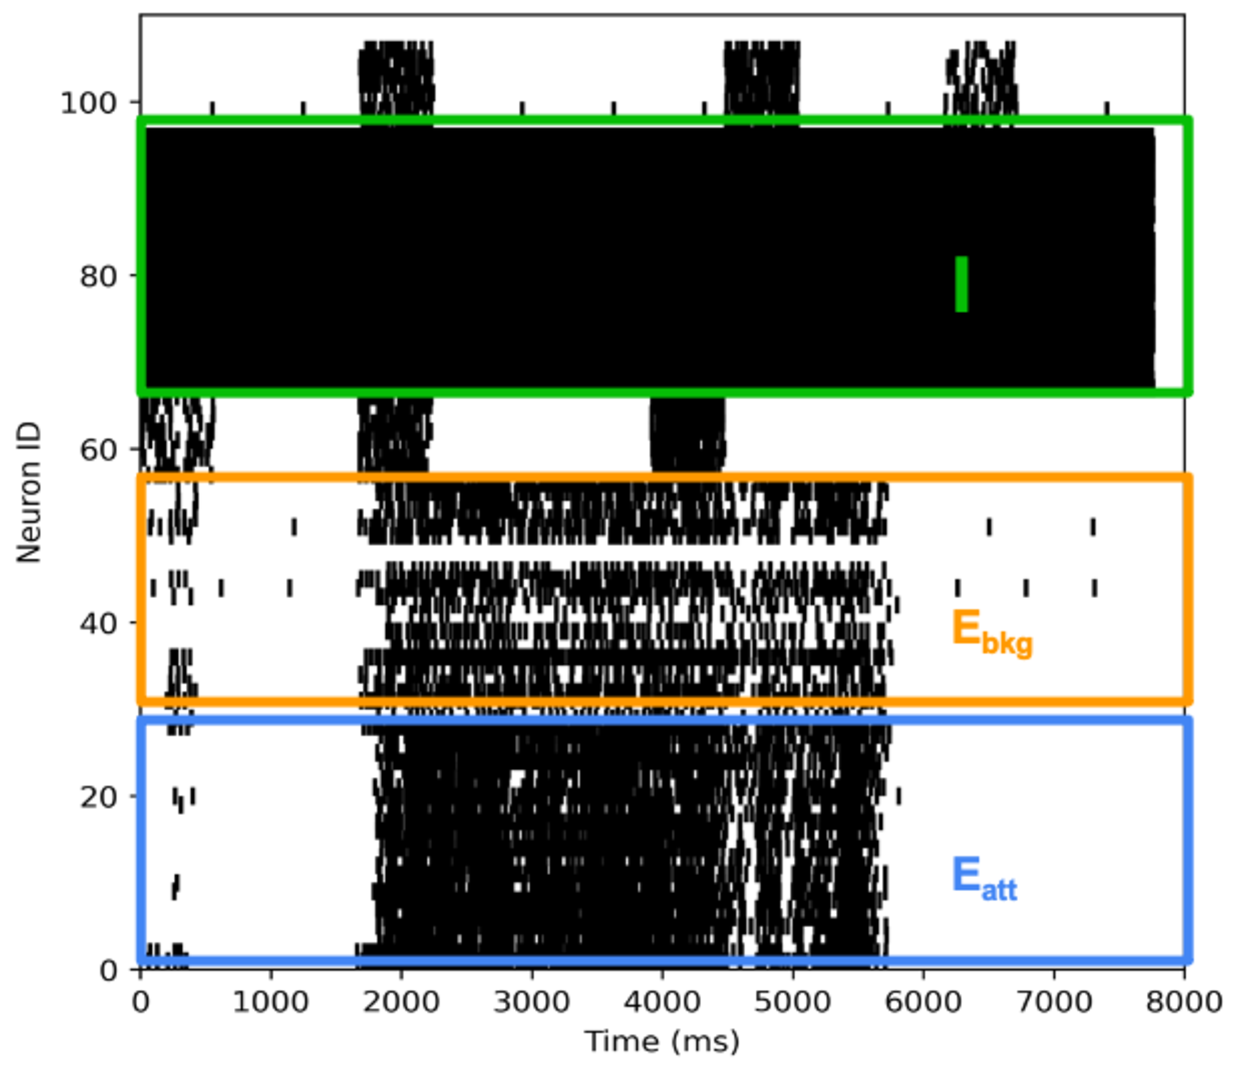
\includegraphics[width=\columnwidth]{./img/behavior/fr_holder.pdf}
		\caption{(b) Raster plot of neuron activities corresponding to input stimuli in (a)}
		\label{fig:neuron_state}
	\end{subfigure}
	\caption{Point attractor behaviour(raster plot) of E population.}
	\label{fig:behavior}
\end{figure}

\begin{figure}
	\begin{subfigure}{\textwidth}
		\centering
		% include first image
		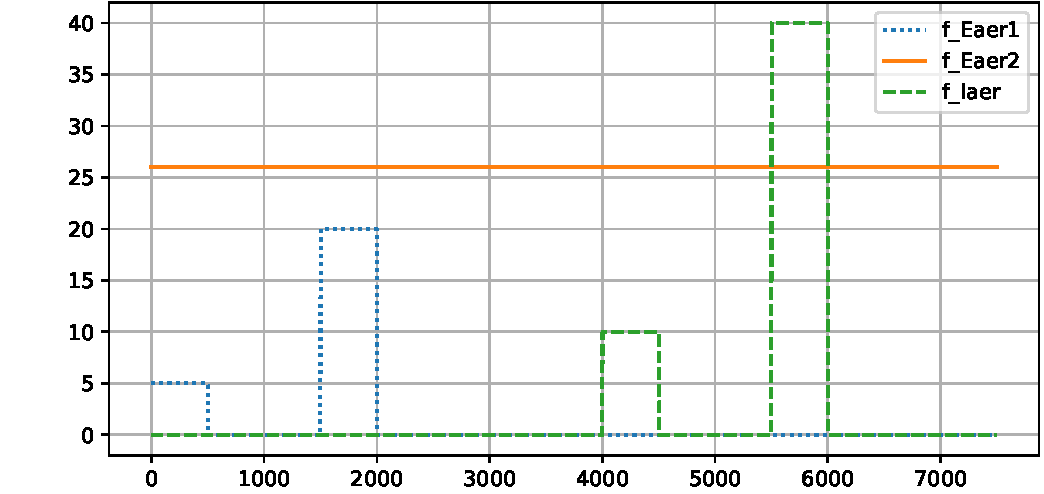
\includegraphics[page=1, width=\columnwidth]{./img/behavior/input_stimuli.pdf}
		\caption{Stimuli of the AER input. (Poisson spike train at different frequencies) (x: time [ms], y: frequency [Hz])}
		\label{fig:spike_input2}
	\end{subfigure}
	\begin{subfigure}{\textwidth}
		\centering
		% include second image
		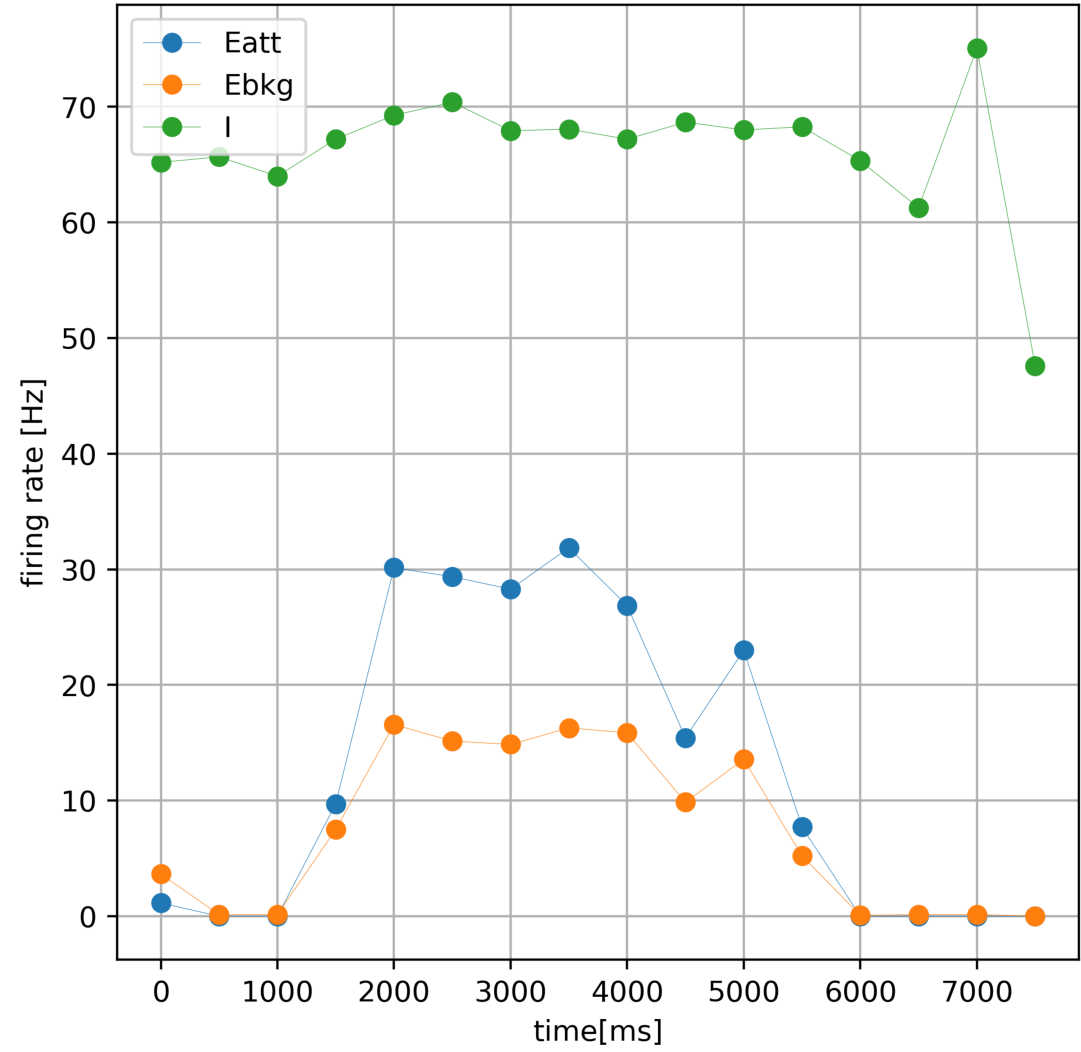
\includegraphics[width=\columnwidth]{./img/behavior/fr_time.pdf}
		\caption{Neuron population point attractor behaviour}
		\label{fig:neuron_state2}
	\end{subfigure}
	\caption{Neuron population point attractor behaviour. At time 0ms, a weak excitation is applied to $E_{att}$ populations, around time 1500ms, a strong excitation is applied to $E_{att}$ population, at time 4000ms, a weak inhibition is applied to the $E_{att}$ population, around time 5500ms, a strong inhibition is applied to the $E_{att}$ populations. }
	\label{fig:behavior2}
\end{figure}

By fine tuning the parameters, a final point attractor state of the E population is obtained as 
shown in figure \ref{fig:behavior}.
The raster plot shows three neuron populations: I, $E_{bkg}$ and $E_{att}$ population. 
To be more clear about the population firing states, the neuron population firing rate is further counted and averaged in figure \ref{fig:behavior2}.\\

As shown in the figure, 
\begin{itemize}
	\item at time 0 ms, a weak excitation is applied to $E_{att}$ populations, the two populations has a firing rate about 3-5 Hz.
	\item at time 1500 ms, a strong excitation is applied to $E_{att}$ populations, $E_{att}$ reaches a firing rate around 30Hz and $E_{bkg}$ reaches a firing rate around 18 Hz.
	\item at time 4000 ms, a weak inhibition is applied to $E_{att}$ populations, both $E_{bkg}$ and $E_{att}$ populations firing rate drop a bit but soon return back around the normal state.
	\item at time 5500 ms, a strong inhibition is applied to $E_{att}$ populations, both $E_{bkg}$ and $E_{att}$ populations firing rate drop to zero.
\end{itemize}

It is believed that the E population neurons reaches a point attractor state where it can only switch to a "high" state with a strong excitatory stimuli, and can be stable when small inhibition or weak perturbation appears. They can only switch back to "low" state by feeding in strong inhibition stimuli.

The excitatory threshold to realise "low" to "high" state is about 5Hz and the inhibitory threshold from "high" to "low" should be larger than 10Hz. The population "high" state is around 30Hz and "low" state is 0Hz.
